\documentclass[11pt]{article}

\usepackage[utf8]{inputenc}
\usepackage{fancyhdr}
\usepackage{hyperref}
\usepackage{graphicx}

\graphicspath{ {images/} }
 
\pagestyle{fancy}
\fancyhf{}
\lhead{University of the Witwatersrand}
\rfoot{School of Computer Science and Applied Mathematics}
\pagenumbering{roman}
\fancyfoot[R]{\thepage}

\begin{document}
\begin{page}

\newcommand{\HRule}{\rule{\linewidth}{0.3mm}} % Defines a new command for the horizontal lines, change thickness here
\renewcommand\section{\@startsection{section}{1}{\z@}%
                                  {-3.5ex \@plus -1ex \@minus -.2ex}%
                                  {2.3ex \@plus.2ex}%
                                  {\normalfont\large\bfseries}}
\setlength{\parindent}{0pt}

\center % Center everything on the page
 
%----------------------------------------------------------------------------------------
%	HEADING SECTIONS
%----------------------------------------------------------------------------------------

\textsc{\LARGE University of the Witwatersrand}\\[1.5cm] % Name of your university/college
\textsc{\Large School of Computer Science and Applied Mathematics}\\[0.5cm] % Major heading such as course name

%----------------------------------------------------------------------------------------
%	TITLE SECTION
%----------------------------------------------------------------------------------------

\HRule \\[0.4cm]
{ \huge \bfseries COMS3008: Parallel Computing Lab Assignment 1}\\[0.4cm] % Title of your document \\
  \large 25 July 2016
\HRule \\[1.5cm]
 
%----------------------------------------------------------------------------------------
%	AUTHOR SECTION
%----------------------------------------------------------------------------------------
\begin{minipage}{1\textwidth}
	\Large \emph By Chalom, J. (711985)\\
\end{minipage}


\vfill % Fill the rest of the page with whitespace

\end{page}

\begin{page}

\clearpage
\setcounter{page}{1}
\pagenumbering{arabic}

\section{General Method Used}
I programmed all experiments in C++. I ran these experiments in a virtual machine with 4GB ram and 4 cores from an i7 4770. The VM ran Ubuntu 16.04. The host system was Windows 10. All results were outputted into CSV formatted files. Further processing was done with another program (included source) which again saved the results obtained into another series of CSV files. I then used Microsoft Excel to produce most of the diagrams in this report.\\

\noindent For all random numbers generated, they were doubles ranging from 0.0 to 100.0, and were generated using the rand() function. The random seed was generated at the start of the main thread.\\

\noindent All timing was done using openMP, and its \texttt{omp\char`_get\char`_wtime()} function. This was done by getting a start time before the desired series of operations and an end time after those operations were completed. A difference was produced which was the time those operations took to complete in seconds.\\

\noindent Part 1 took: 970.991269 seconds to complete.\\
Part2 took: 1.398433 seconds to complete.\\
Part 3 took: 29864.678942 seconds to complete.\\


\section{Accessing multi-dimensional arrays}
\begin{figure}[ht]
\centering
     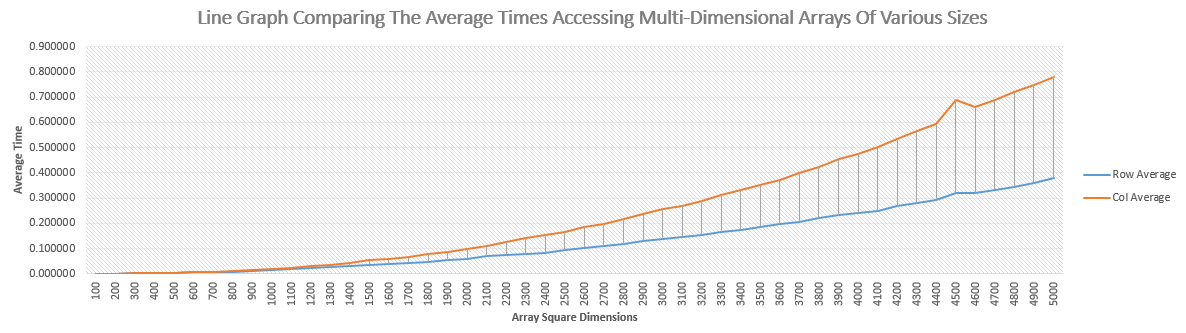
\includegraphics[width=1.0\textwidth]{Example1_Avg}
     Line Graph Comparing The Average Times Accessing Multi-Dimensional Arrays Of Various Sizes\\
\end{figure}

\noindent \chapter{Method:}
In this experiment I used 2D pointer arrays that were dynamically allocated. This enabled me to literately increase the dimensions of the arrays I was testing - in a square manner. For each dimensional increase I repeated the timed experiment 50 times and from the results generated the average for each 50 ‘block’, and also found the min, max, range and variance for that ‘block’. I repeated the experiment until the dimensions of the array went up to 5000 X 5000.\\

\noindent \chapter{1.0 Observation:}\\
I observed in this experiment and from the resulting diagram (above) that the relationship between accessing a 2D array by row first or by column first is very interesting. There is an exponential trend occurring in the times as the dimensions of the arrays increase. Row dominant algorithms also seem to be faster.\\

\noindent \chapter{1.1 Reasons for differences in access times:}\\
The reason for the difference in access times between row dominant and column dominant comes from how an array of pointers is stored in memory.

\begin{figure}[ht]
\centering
     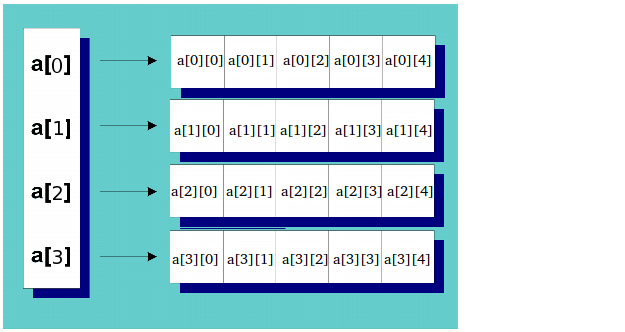
\includegraphics[width=1.0\textwidth]{M75kn}
     Source: \url{http://stackoverflow.com/questions/936687/how-do-i-declare-a-2d-array-in-c-using-new}\\
\end{figure}

\noindent Memory of the system is not multi-dimensional. It is very flat in nature. A dynamically allocated pointer array in the method done in the code for this assignment will therefore be split up into rows and placed in the nearest available memory space. The Diagram above shows this process and what the references of the different rows of the array look like. By accessing column first the code is making the system jump between these different dis-contiguous memory spaces storing each row ‘chunk’. This is much slower due to the increase in memory access operations than loading a row where each individual data point is next to each other. Row first allows for better caching and a jumping operation only after each row rather than each data point as in the column first algorithm.\\

\noindent I attempted to test statically allocated arrays. Unfortunately I was unable to implement a test environment to iterate through a series of different dimensions because these arrays are statically assigned at start-up. What happens here is that a memory space that is able to store the whole array is chosen thereby not breaking up the array into parts. 

\begin{figure}[ht]
\centering
     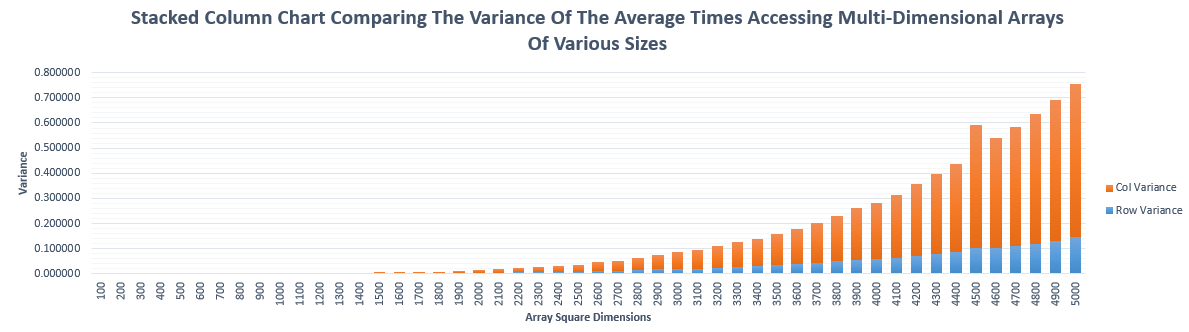
\includegraphics[width=1.0\textwidth]{Example1_Var}
     Stacked Column Chart Comparing The Variance Of The Average Times Accessing Multi-Dimensional Arrays Of Various Sizes 

\end{figure}

\noindent This graph reinforces that both sets of average elapsed time intervals for row and column exponentially increase.

\section{Display output from threads}
\noindent \chapter{Method:}
For this experiment I locked the number of threads to 10 threads. I then outputted to file the thread numbers as they executed. This was then repeated 100 times. I then generated the image above by assigning a colour to each number and plotting an image going down (for each iteration of the experiment) where each pixel is the specific thread executed in order. I used an image processing tool I made. Which can be found here: \url{ https://github.com/TRex22/SkunkworksImageProcessor}

\noindent \chapter{Observation:}
The image seems mostly random with some patterns emerging where the same process was executed in the same position for a while before being changed.

\noindent \chapter{Reason for the order switching:}
There could be many reasons for why the order switches. Most likely it is the operating system scheduling tasks. Since no locking is specified there is a race condition set up where whichever thread is first is able to write to file. Due to this it is likely for the same thread to occur in the same place in the execution cycle due to interference from the OS, however a more random system should be produced in general due to all the threads except the main are identical.\\

\noindent I believe that my use of a virtual machine may have affected the results as the host system my affect what processors, real or logical are assigned to the VM and may even change the resources without the internal OS knowing about it. This could affect the results. It is also likely that optimisations in the VM software also affected the results.


\section{Vector dot product}
\noindent \chapter{Method:}
For the first part which was to vary the number of threads being used to calculate the dot product of two randomly generated vectors. I iteratively did this from 1 to 1000 threads. I fixed the vector size to 5000000. I repeated each iteration 50 times and wrote the results to file. Later I calculated statistics on the results.\\

\noindent For the second part I kept the number of threads to 4 (the number of logical processors the VM had) and iteratively increase the vector dimensions up to 1000. I also did each iteration 50 times and later worked out statistics on the results.

\begin{figure}[ht]
\centering
     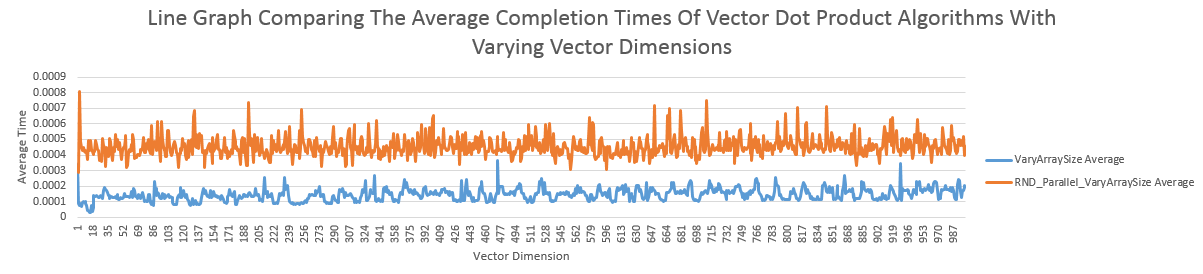
\includegraphics[width=1.0\textwidth]{Example3_Dimension}
     Line Graph Comparing The Average Completion Times Of Vector Dot Product Algorithms With Varying Number Of Threads\\
\end{figure}

\noindent \chapter{1.1	Effect of varying the number of threads:}
I found this to significantly slow down the execution time versus fixing the number of threads. This is probably due to interference caused by the VM. Another reason could be that there is a lot of context switching of the different threads by the OS which introduces latency – removing the benefit of parallelizing the algorithm.\\

\noindent \chapter{1.2	Effect of varying size of the vectors:}
I found this to be significantly faster. Most likely due to the system having the least amount of context switching due to the number of threads equalling the number of logical cores of the VM. Another reason could be to caching and optimization due to the VM or OS.\\

\noindent \chapter{1.3 Effect of parallelizing random number generation:}
The effect shown was much higher variance of the results as well as much higher results on average compared to where the random number generation was not parallelized. Again by having more sub-threads the cost of context switching and waiting / idle will increase, and I believe this is what made the algorithms slower to complete.\\

\begin{figure}[ht]
\centering
     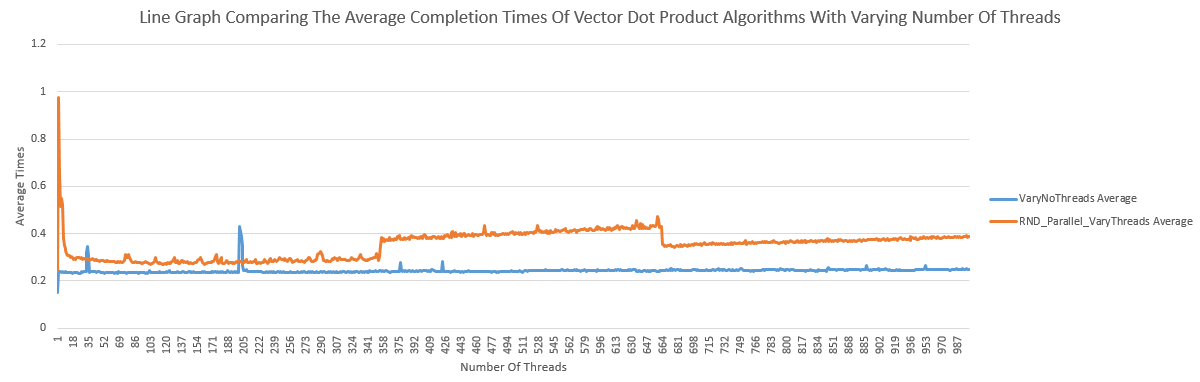
\includegraphics[width=1.0\textwidth]{Example3_Threads}
     Line Graph Comparing The Average Completion Times Of Vector Dot Product Algorithms With Varying Vector Dimensions\\
\end{figure}

\end{page}
\end{document}
